\chapter{Referencial Teórico}

Neste capítulo apresentaremos uma revisão da literatura agrupando trabalhos relacionados a reprovações e dificuldades de alunos em disciplinas de programação, novas abordagens de ensino e sistemas de dicas. 

\section{Reprovações em Disciplinas de Programação}

O entendimento e aplicação dos conceitos estudados em disciplinas de programação é fundamental para que o aluno consiga desenvolver programas mais complexo. \citeonline{Helminen:2010:JPV:1879211.1879234} afirmam que a programação é uma competência essencial no curso de Ciência da Computação. Segundo \citeonline{bosse2015reprovaccoes} os estudantes normalmente apresentam uma grande dificuldade com os conteúdos abordados, ocasionando em reprovação ou desistência.

% TODO: Completar com os dados do estudo
\citeonline{Sinclair:2015:MSE:2729094.2742586} agruparam pesquisas internacionais como a \textit{National Survey of Student Engagement} (NSSE) feita na América do Norte e Canadá e a pesquisa \textit{Nacional Universidade Experience} (UES). Esse estudo reúne dados relacionadas à Ciência da Computação sendo que os resultados desta meta-análise indicam que o curso de Ciência da Computação apresenta taxas mais baixas do que a média em muitos dos principais pontos de referência de engajamento. A \cref{tabela:NSSEbenchmark} apresenta um resumo das pontuações dos indicadores do NSSE 2013 sendo o máximo de 60 pontos para cada indicador e quanto maior melhor. Assim, a pontuação do curso de Ciência da Computação estão abaixo da média geral para todas as categorias exceto Collaborative Learning em que é igual. Em vários indicadores, o curso de Ciência da Computação está apenas 1 ou 2 pontos (em 60) trás, mas em \textit{Reflective Learning} e \textit{Learning Strategies} em particular, a diferença é maior. Em ambos esses indicadores as Ciências Físicas e Engenharia são geralmente de baixa pontuação e pode ser considerado como comparações sujeitas próximos do curso de Ciência da Computação. 

\begin{table}[]
	\centering
	\captionsetup{justification=centering}
	\caption{Indicadores da pesquisa NSSE 2013, com fonte em \cite{Sinclair:2015:MSE:2729094.2742586}}
	\label{tabela:NSSEbenchmark}
	\begin{tabular}{|l|c|c|c|c|}
		\hline
		\textbf{Subject Area}           & \multicolumn{1}{l|}{\textbf{CS}} & \multicolumn{1}{l|}{\textbf{Phys. Sci.(not CS)}} & \multicolumn{1}{l|}{\textbf{Eng}} & \multicolumn{1}{l|}{\textbf{Overall}} \\ \hline
		Higher Order Learning           & 38                               & 40                                               & 39                                & 39                                    \\ \hline
		Reflective Learning             & 32                               & 34                                               & 33                                & 39                                    \\ \hline
		Learning Strategies             & 34                               & 39                                               & 36                                & 41                                    \\ \hline
		Quantitative Reasoning          & 28                               & 38                                               & 37                                & 29                                    \\ \hline
		Collaborative Learning          & 32                               & 36                                               & 40                                & 32                                    \\ \hline
		Discussions with Diverse Others & 38                               & 41                                               & 41                                & 41                                    \\ \hline
		Student Faculty Interaction     & 20                               & 28                                               & 23                                & 24                                    \\ \hline
		Student Faculty Interaction     & 37                               & 41                                               & 38                                & 41                                    \\ \hline
		Quality of interactions         & 42                               & 43                                               & 41                                & 43                                    \\ \hline
		Supportive environment          & 31                               & 34                                               & 32                                & 33                                    \\ \hline
	\end{tabular}
\end{table}

A \cref{tabela:UESbenchmark} apresenta um resumo dos resultados da UES. Das categorias gerais nos UES, o curso de Ciência da Computação apresenta mal resultados em duas: segundo mais baixo no \textit{Skills Development} em comparação dentro das 45 áreas específicas, e décimo mais baixo em \textit{Teach Quality}. Outras categorias apresentam melhores resultados, sendo uma acima da média para \textit{Learner Engagement} e também \textit{Student Support} e apenas dois abaixo da média para \textit{Learning Resource}.

\begin{table}[]
	\centering
	\captionsetup{justification=centering}
	\caption{Resumo dos resultados da UES, com fonte em \cite{Sinclair:2015:MSE:2729094.2742586}}
	\label{tabela:UESbenchmark}
	\begin{tabular}{|l|c|c|c|c|c|}
		\hline
		\multicolumn{1}{|c|}{\textbf{Subject Area}} & \textbf{Skills Dev} & \textbf{\begin{tabular}[c]{@{}c@{}}Learner \\ Engagement\end{tabular}} & \textbf{Teach Quality} & \textbf{\begin{tabular}[c]{@{}c@{}}Learning \\ Resource\end{tabular}} & \textbf{\begin{tabular}[c]{@{}c@{}}Student \\ Support\end{tabular}} \\ \hline
		CS                                          & 72                  & 58                                                                     & 74                     & 81                                                                    & 54                                                                  \\ \hline
		Overall                                     & 79                  & 57                                                                     & 79                     & 83                                                                    & 53                                                                  \\ \hline
	\end{tabular}
\end{table}

\section{Novas Técnicas de Ensino}

\citeonline{Knobelsdorf:2014:TTC:2538862.2538944} aplicaram uma abordagem cognitiva de aprendizagem no curso teórico realizado na Universidade de Potsdam, na Alemanha, e têm levado a uma redução significativa das taxas de falha do curso. O objetivo era tornar as práticas do curso teórico de Ciência da Computação mais visíveis aos alunos e, portanto, mais fáceis de adotar. Reforçaram a modelagem introduzindo uma sessão tutorial, que consiste em apresentar as habilidades para manusear e trabalhar com o conhecimento que os alunos devem desenvolver no curso. Aplicaram o método \textit{Scaffolding \& Fading}, onde foi oferecido exercícios preparatórios específicos que devem ser resolvidos em conjunto durante a sessão de exercícios e servem como preparação para o dever de casa. E por fim, forneciam \textit{feedback} para as submissões e trabalhos de casa realizados pelos alunos. Para avaliar a nova abordagem, foi realizado um exame final mantendo os mesmos requisitos das versões dos útimos 5 anos e obteram uma taxa de insucesso inferior a 10\% em dois anos consecutivos que antes alcançava de 30 a 60\%.

\citeonline{Cukierman:2015:PSU:2729094.2742623} realizou estudos experimentais para determinar se novas atividades em sala de aula, como a instrução entre pares ea aprendizagem ativa, auxiliada pelo uso de sistemas de resposta do público (i-clickers) utilizado em palestras e o Programa de Aperfeiçoamento Acadêmico (AEP), que consiste na intervenção pró-activa centrada nos estudantes desenvolvida e gerida pela \foreign{School of Computing Science and Student Learning Commons} na Universidade \foreign{Simon Fraser}, proporcionando oportunidades de auto-reflexão e exposição a estratégias de estudo melhoram em algumas medidas de resultado (tais como notas de exame final). Para realizar o experimento, foram definicas as seguintes variáveis:

\begin{itemize}
	\item \textbf{AEP}: Participação em atividades da AEP. Este é um predictor dicotômico que indica se os alunos participaram (codificados como 1) ou não (codificados como 0) nas atividades da AEP.
	
	\item \textbf{MID}: pontuações de meio termo. Este é um preditor contínuo, variando de 0 a 100.
	
	\item \textbf{WIC}: Participação ponderada do I-clicker. Este é um predictor contínuo que mede a participação do i-clicker que varia de 0 a 100 e calculado acumulando pontos de todas as conferências quando i-clickers foram usados. Nessas palestras, os pontos foram baseados incluindo a participação e resposta correta de perguntas no i-clicker.
	
	item \textbf{FIN:}: Pontuações finais do exame. Este é o critério contínuo ou variável de resultado, que varia de 0 a 100.
\end{itemize}

\begin{figure}[]
	\centering
	\captionsetup{justification=centering}
	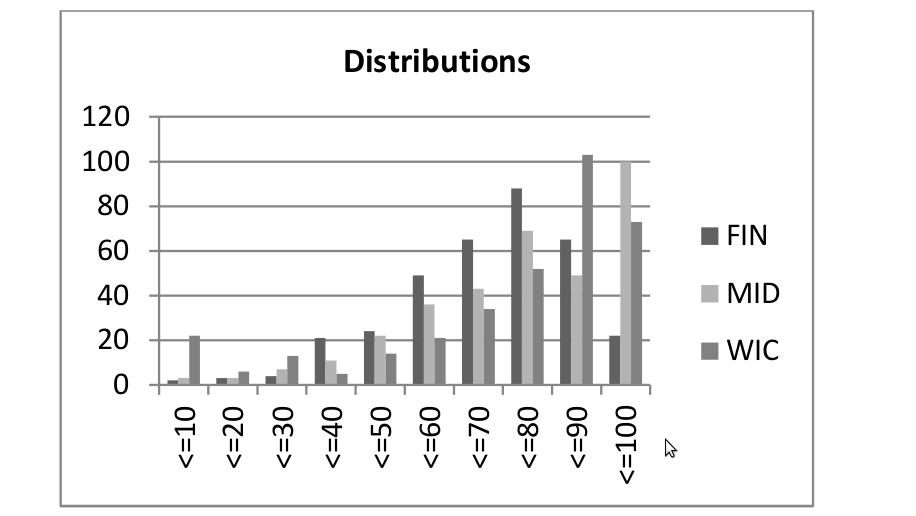
\includegraphics[width=.8\linewidth]{referencialteorico/cukierman.png}
	\caption{Distribuições de FIN, MID e WIC. O gráfico não inclui os alunos que se retiraram do curso, nem com FIN = 0. Fonte \cite{Cukierman:2015:PSU:2729094.2742623}}
	\label{figura:resultadoCukierman}
\end{figure}

A \cref{figura:resultadoCukierman} a presenta o resultado obtido na pesquisa, sendo que o estudo não incluiu alunos que se retiraram do curso ou não vieram para o exame final. Intuitivamente, os alunos tiveram um desempenho muito bom no meio termo, com um grande número de alunos com mais de 90\%. Os alunos obtiveram valores muito bons nos pontos ponderados do i-clicker e no exame final pode-se observar que os resultados são mais distribuídos, embora negativamente inclinados.


\section{Mecanismo de Dicas}

Nas abordagens citadas a baixo, uma dica equivale a um auxílio ao aluno para que ele consiga realizar um exercício que esteja com dificuldade, essa dica pode ser oferecida tanto pelo professor ou colega de turma. Um sistema que utiliza esse conceito pode ser chamado de sistema de dicas, onde reproduz esse contato que o aluno teria com uma pessoa mais instruída quando precisa tirar uma dúvida ou pedir uma dica para realizar o exercício. Mas o aluno com dificuldades não pode ter esse apoio todo o tempo, então estão sendo criados sistema de dicas para suprir essa necessidade de auxiliar o aluno no seu aprendizado.

\citeonline{Elkherj:2014:SSR:2556325.2567864} apontam que as sugestões utilizadas em sistemas de aprendizagem on-line para ajudar os alunos quando eles estão tendo dificuldades são fixados antes do tempo e não dependem das tentativas mal sucedidas que o aluno já fez. Isto limita severamente a eficácia das sugestões. Eles desenvolveram um sistema alternativo para dar dicas aos estudantes. A principal diferença é que o sistema permite um instrutor enviar uma dica para um estudante após o aluno ter feito várias tentativas para resolver o problema e falhou. Depois de analisar os erros do aluno, o instrutor é mais capaz de entender o problema no pensamento do aluno e enviar-lhes uma dica mais útil. O sistema foi implantado em um curso de probabilidade e estatística com 176 alunos, obtendo \textit{feedback} dos alunos muito positivo. Mas o desafio que os autores enfrentam é como escalar efetivamente o sistema de forma que todos os alunos que precisam de ajuda obtenham dicas eficazes. Pois com uma grande quantidade de alunos ficaria exaustivo para os instrutores avaliarem cada submissão dos exercícios de cada aluno para retornarem uma dica especifica do erro cometido. Então eles criaram um banco de dados de dica que permite que os instrutores reutilizem, compartilhem e melhorem em cima de sugestões escritas anteriormente.

\citeonline{Price:2015:IIF:2787622.2787748} está utilizando um sistema de tutores inteligentes (STI) que podem manter os alunos no caminho certo, na ausência de instrutores, fornecendo sugestões e advertências para os alunos que precisam de ajuda. Além disso, as técnicas baseadas em dados podem gerar feedback automaticamente a partir de tentativas de resolução de um problema. O autor está aplicando o seu estudo permitindo que os alunos escrevam códigos que se conectam com seus interesses, tais como jogos, aplicações e histórias. Como exemplo concreto, imagine um aluno que esteja desenvolvendo um jogo simple, quer requer a utilização de variáveis, laços de repetição, condicionais. Mas o aluno está com dificuldades em relação a uma funcionalidade que o jogo terá, ele poderá pedir uma dica para implementar essa funcionalidade que será gerada automaticamente pelo sistema com relação as tentativas anteriores de outros alunos.

\citeonline{Cummins:2016:IUH:2876034.2893379} investigaram  o uso de dicas para 4.652 usuários qualificados em um ambiente de aprendizagem on-line de grande escala chamado Isaac, que permite aos usuários para responder a perguntas de física com até cinco dicas. Foi investigado o comportamento do usuário ao usar dicas, engajamento dos usuários com desvanecimento (o processo de tornar-se gradualmente menos dependentes das dicas fornecidas), e estratégias de dicas incluindo decomposição, correção, verificação ou comparação. Como resultados obtidos, os alunos apresentaram estratégias para as resoluções dos exercícios sendo a mais comum é ver o conceito da dica para realizar a decomposição do problema e, em seguida, enviar uma resposta correta. A outra estratégia é usar os conceitos da dica para determinar se a pergunta pode ser respondida, uma grande proporção dos usuários que utilizaram essa estratégia acabou não tentando responder a pergunta


\section{Considerações Finais}
%- fazer um resumo das abordagens de ensino e o engajamento dos estudantes
%criar um capitulo de sumarização dos artigos relacionados e comentar o porque de usar o sistema de dicas que vou criar.
%- consideraçoes finais 
%	- juntar tudo e falar o porque do meu tcc